\documentclass[8.01x]{subfiles}
\begin{document}

\chapter{Week 9: Homework 7}

\section{Problem 1: Rotational kinematics: turntable solutions}

``A turntable is a uniform disc of mass $m$ and radius $R$. The turntable is initially spinning clockwise when looked down on from above at a constant frequency $f_0$. The motor is turned off at $t = 0$ and the turntable slows to a stop in time $t$ with constant angular deceleration.

(a) What is the magnitude of the initial angular velocity $\omega_0$ of the turntable? Express your answer in terms of $f_0$.\\
(b) What is the magnitude of the angular acceleration $\alpha$ of the turntable? Express your answer in terms of $f_0$ and $t$.\\
(c) What is the magnitude of the total angle $\Delta \theta$ in radians that the turntable spins while slowing down? Express your answer in terms of $f_0$ and $t$.''

Writing down the answers will likely take longer than it takes to solve these questions! We can use the simple equations for rotational kinematics that we saw in the beginning of lecture 19. One was not mentioned there, which is

\begin{equation}
f_0 = \frac{1}{T} = \frac{\omega}{2 \pi}
\end{equation}

This implies that $\omega = 2 \pi f_0$, which answers part (a).

For part (b), we use $\displaystyle \alpha = \frac{\omega_1 - \omega_0}{\Delta t}$, where $\omega_0$ is the initial angular velocity, and $\omega_1$ the final angular velocity.

In this case, $\omega_0 > \omega_1$, so $\alpha$ is negative. However, they asked for the magnitude, so we drop the sign, and it comes to a complete halt at time $t$, so $\omega_1 = 0$:

\begin{equation}
\alpha = \frac{\omega_0}{t} = \frac{2 \pi f_0}{t}
\end{equation}

Finally, for part (c), we can use $\Delta \theta = \omega_0 t + \frac{1}{2} \alpha t^2$, derived from $\displaystyle \theta = \theta_0 + \omega_0 t + \frac{1}{2} \alpha t^2$. $\alpha$ is negative, so the addition becomes a subtraction:

\begin{equation}
\Delta\theta = 2 \pi f_0 t - \frac{1}{2} \left(\frac{2 \pi f_0}{t}\right) t^2 = 2 \pi f_0 t - \left(\pi f_0\right) t = \pi f_0 t
\end{equation}

That's it!

\section{Problem 2: Angular dynamics}

``A playground merry-go-round has a radius of $R = 2$  m and has a moment of inertia $I_{cm} = \SI{5e3}{kg m^2}$ about a vertical axis passing through the center of mass. There is negligible friction about this axis. Two children each of mass $m = 25$ kg are standing on opposite sides at a distance $r_o = 1.4$ m from the central axis. The merry-go-round is initially at rest. A person on the ground applies a constant tangential force of $F = \SI{2e2}{N}$ at the rim of the merry-go-round for a time $\Delta t = 10$ s . For your calculations, assume the children to be point masses.

\begin{center}
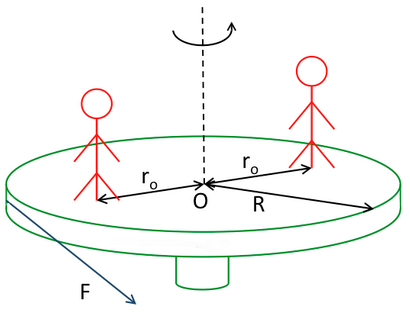
\includegraphics[scale=0.65]{Graphics/h7p2}
\end{center}

(a) What is the angular acceleration $\alpha$ of the merry-go-round (in $\text{rad/s}^2$)?\\
(b) What is the angular velocity $\omega_{final}$ of the merry-go-round when the person stopped applying the force (in rad/s)?\\
(c) What average power $P_{avg}$ does the person put out while pushing the merry-go-round (in Watts)?\\
(d) What is the rotational kinetic energy R.K.Efinal of the merry-go-round when the person stopped applying the force (in $\text{kg m}^2/\text{s}^2$)?''

Hmm, I wonder if there is a particular reason why part (d) is not in joules. The dimension is equivalent, but they didn't state ``in joules'' for whatever reason.

Anyhow, let's see. Unless otherwise specified, I will consider torques and angular momentum relative to the center of mass -- though angular momentum should be the same for all points, since this is a rotation about the center of mass, so that disclaimer is probably not necessary.

To start with, we need to calculate the moment of inertia, since we only know it without the children being included.\\
Considering them as point masses, the total moment of inertia is just the sum of $I_{cm}$ plus $m r_o^2$ for each of the children:

\begin{equation}
I = I_{cm} + 2 m r_o^2 = \SI{5098}{kg m^2}
\end{equation}

Now, then. The rotational analogue of $F = m a$ is $\tau = I \alpha$. We can find $\alpha$ very easily if we only find the torque relative to the center of mass.\\
The torque is given by $\tau = \vec{R} \times \vec{F}$, where $\vec{R}$ is the position vector from the origin to point where the force is applied. The force is specified as ``tangential'', so there is always a right angle between the two, and $\vec{R} \times \vec{F} = R F$, since $\sin(\pi/2) = 1$. The angular acceleration is then

\begin{equation}
\alpha = \frac{\tau}{I} = \frac{R F}{I} = \SI{0.0785}{rad/s^2}
\end{equation}

Using that, we can find the final angular velocity very easily, using $\omega = \omega_0 + \alpha t$. $t$ is given as 10 seconds in this case, so

\begin{equation}
\omega_{final} = 0 + \alpha t = \SI{0.785}{rad/s}
\end{equation}
In more familiar units, this is 8.00 seconds per rotation (0.125 Hz or 7.5 rpm).

What is the average power of the person pushing the merry-go-round? We should be able to use $W = \vec{F} \cdot \vec{v}$ here, where $v$ is the tangential velocity, $v = \omega R$. The two are always parallel, and so

\begin{equation}
P = F v = F \omega R
\end{equation}

We could find the average using an integral: 

\begin{equation}
P_{avg} = \frac{1}{t_b - t_a} \int_{t_a}^{t_b} P(t) \mathop{dt}
\end{equation}

... but surely there is a better way. I looked up the relationship for power and torque, and found that $P = \vec{\tau} \cdot \vec{\omega}$, which also would require an integration (in fact, it would be the same integral), since $\omega$ is constantly changing.

I'm not sure if there is an easier way, but this integral shouldn't be very bad, so let's do it.

\begin{align}
P_{avg} &= \frac{1}{\Delta t} \int_{0}^{\Delta t} F R \omega(t) \mathop{dt}\\
        &= \frac{F R}{\Delta t} \int_{0}^{\Delta t} \alpha t \mathop{dt}\\
        &= \frac{F R \alpha}{\Delta t} \left(\frac{(\Delta t)^2}{2}\right)\\
        &= \frac{F R \alpha \Delta t}{2}
\end{align}

For these values, $P_{avg} = 157$ watts. Quite reasonable.

And at last, the final rotational kinetic energy. The book proves that the work-energy theorem is applicable to rotational energy, so all the work done ($W = P_{avg} \Delta t$) is turned into rotational kinetic energy, so the answer is 

\begin{equation}
W = P_{avg} \Delta t = \SI{1570}{J}
\end{equation}

As as update after the staff solutions are out, this was technically incorrect -- but was accepted anyway. They wanted the rotational kinetic energy of the \emph{merry-go-round alone, without the children}, but I don't think that was too clear.\\
We can find the kinetic energy of that alone as $\displaystyle \frac{1}{2} I_{cm} \omega^2 \approx 1540$ J, instead. Not a lot harder, but I do think the question is a bit vague. Since the previous three questions were all found by considering the children's moments of inertia, I just assumed we should do here, too.

\section{Problem 3: Atwood machine}

``A pulley of mass $m_p$, radius $R$, and moment of inertia about the center of mass $\displaystyle I_c = \frac{1}{2} m_p R^2$, is suspended from a ceiling. The pulley rotates about a frictionless axle. An inextensible string of negligible mass is wrapped around the pulley and it does not slip on the pulley. The string is attached on one end to an object of mass $m_1$ and on the other end to an object of mass with $m_2 < m_1$.

At time $t = 0$, the objects are released from rest.

\begin{center}
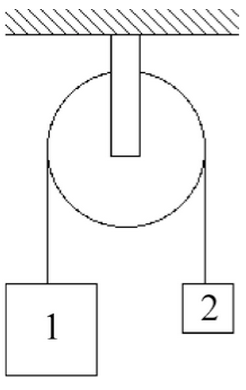
\includegraphics[scale=0.65]{Graphics/h7p3}
\end{center}

(a) Find the magnitude of the acceleration of the two objects. Express your answer in terms of $m_1$, $m_2$, $m_p$, $R$ and acceleration due to gravity $g$.\\
(b) How long does it take the objects to move a distance $d$? Express your answer in terms of $m_1$, $m_2$, $m_p$, $d$ and acceleration due to gravity $g$.''

Ah, interesting stuff: a non-massless pulley! Granted, we don't allow for any slipping, and the string is still of negligible mass... but this is still a considerable step towards some realism.\\
The string is \emph{not massless}, however. Remember that when a string is massless, we can prove that the tension at two different points along the string must have the same magnitude... but in this case, a difference in tension is the cause of the torque that rotates the pulley! More on that in a second.

First off, since the string is inextensible, the acceleration and velocity of both masses and the rope (and the pulley, i.e. the tangential velocity at its edge) must all be the same.\\
Since $m_1 > m_2$, the system will accelerate such that $m_1$ goes downwards, $m_2$ upwards, and the pulley rotates counterclockwise, as seen from the direction we see it. This means $\vec{\omega}$ for the pulley will be out of the screen.

The forces on each block are easy to find. Each block has gravity and tension acting on it. I will take downwards to be the positive direction for block 1, and upwards for block 2, which then yields a common acceleration $a$ without any trouble with signs and directions.\\
Let's then write Newton's second law equations for the two blocks:

For block 1, $m_1 a = m_1 g - T_1$.\\
For block 2, $m_2 a = T_2 - m_2 g$.

The differences in tension will cause a tangential force on the pulley, which causes a torque relative to its center, which I will call point C. This torque causes a rotation via $\tau_C = I \alpha_C$.\\
$a = \alpha_C R$ (this is just the time derivative of $v = \omega R$), so we can also say that $\displaystyle \tau = \frac{I a}{R}$, so that $\displaystyle a = \frac{\tau R}{I}$. The dimension works out to be that of acceleration, which is always a good sign!

What is the torque, then? Well, the tension is tangential, and so the moment arm into the center becomes the radius $R$, and the angle is always 90 degrees. That gives us $\tau_C = (T_1 - T_2) R$.\\
We know that the rotation will be counterclockwise, so the torque must be directed out of the screen. Using $\vec{R} \times \vec{F}$ where $F = T_1 - T_2$ with a leftwards direction, the direction of positive torque, according to the cross product, is out of the screen -- as it should be! (That is assuming that $T_1 > T_2$, which it should be in this case.)

This means we have three equations and three unknowns:

\begin{align}
m_1 a &= m_1 g - T_1\\
m_2 a &= T_2 - m_2 g\\
a &= \frac{2(T_1 - T_2)}{m_p}
\end{align}

I substituted in $\displaystyle I = \frac{1}{2} m_p R^2$ in the last equation, which removed the dependence on $R$.

I'm never a fan of solving systems of three equations. Can we simplify the task? Solving the first two for $T_1$ and $T_2$ respectively, we can find $T_1 - T_2$ by subtracting the other sides of those equations:

\begin{equation}
T_1 - T_2 = m_1 g - m_1 a - m_2 a - m_2 g
\end{equation}

We can then stick this into the third equation, and solve for $a$:

\begin{align}
a &= 2 \frac{g(m_1 - m_2) - a (m_1 + m_2)}{m_p}\\
a \left(1 + \frac{2 (m_1 + m_2)}{m_p}\right) &= 2 \frac{g(m_1 - m_2)}{m_p}\\
a &= 2 \frac{g(m_1 - m_2)}{m_p} \frac{1}{\left(1 + \frac{2 (m_1 + m_2)}{m_p}\right)}\\
a &= 2 \frac{g(m_1 - m_2)}{m_p + 2 (m_1 + m_2)} 
\end{align}

Not bad!

Next up, how long does it take to move a distance $d$? $a$ is clearly constant, since there are only constants in the above equation. Therefore, we can use $\displaystyle d = v_0 t + \frac{1}{2} a t^2$ here. $v_0 = 0$, so the first term disappears. We solve the rest for $t$:

\begin{align}
\frac{1}{2} a t^2 &= d\\
t^2 &= \frac{2 d}{a}\\
t &= \sqrt{\frac{2 d}{a}}
\end{align}

All that remains is then to stick the above, semi-complex expression into the square root:

\begin{align}
t &= \sqrt{\frac{2 d}{2 \frac{g(m_1 - m_2)}{m_p + 2 (m_1 + m_2)}}}\\
t &= \sqrt{d \cdot \frac{m_p + 2 m_1 + 2 m_2}{g(m_1 - m_2)}}
\end{align}

\section{Problem 4: Pulley-object rotational dynamics}

``A light inflexible cable is wrapped around a cylinder of mass $m_1$, radius $R$, and moment of inertia about the center of mass $I_c$. The cylinder rotates about its axis without friction. The cable does not slip on the cylinder when set in motion. The free end of the cable is attached to an object of mass $m_2$. The object is released from rest at a height $h$ above the floor. You may assume that the cable has negligible mass. Let $g$ be the acceleration due to gravity.

\begin{center}
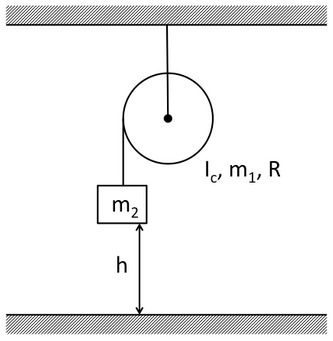
\includegraphics[scale=0.65]{Graphics/h7p4}
\end{center}

(a) Find the acceleration $a$ of the falling object. Express your answer in terms of $m_2$, $R$, $I_c$ and $g$.\\
(b) Find the tension $T$ in the cable. Express your answer in terms of $m_2$, $R$, $I_{cm}$ and $g$.\\
(c) Find the speed $v$ of the falling object just before it hits the floor. Express your answer in terms of $m_2$, $R$, $I_{cm}$, $h$ and $g$.''

Hmm, this looks as if it should be easier than the previous problem.\\
The cable has negligible mass, so the tension ought to be zero without the mass there. Therefore, the tension is all due to gravity acting on the block.\\
Newton's second low on the block, taking downwards to be positive, is

\begin{equation}
m_2 a = m_2 g - T
\end{equation}

The tension then acts on the pulley, in a tangential fashion (as in the last problem, though on the side this time, instead of the top), so that the torque relative to its center is $\tau_C = \vec{R} \times \vec{T} = R T$, with the direction being out of the screen (since the rotation will be counterclockwise). $\vec{R}$ is then the position vector from the center to the point where the force acts, so the $\sin \theta$ term is again always 1, due to the 90 degree angle between the two vectors.

This torque causes an acceleration of the pulley via

\begin{equation}
\tau_C = I_c \alpha \Rightarrow \alpha = \frac{\tau_C}{I_c} = \frac{R T}{I_c}
\end{equation}

$\displaystyle a = \alpha R \Rightarrow \alpha = \frac{a}{R}$, so

\begin{align}
\frac{a}{R} &= \frac{R T}{I_c}\\
a &= \frac{R^2 T}{I_c}
\end{align}

Two equations, with $a$ and $T$ as two unknowns. We can solve both for $a$, sen them equal, and find $T$:

\begin{align}
g - \frac{T}{m_2} &= \frac{R^2 T}{I_c}\\
\frac{T}{m_2} &= g - \frac{R^2 T}{I_c}\\
T + \frac{m_2 R^2 T}{I_c}&= m_2 g\\
T \left(1 + \frac{m_2 R^2}{I_c}\right) &= m_2 g\\
T &= m_2 g \frac{1}{\left(1 + \frac{m_2 R^2}{I_c}\right)}\\
T &= \frac{m_2 g}{1 + \frac{m_2 R^2}{I_c}}\\
T &= \frac{m_2 g I_c}{I_c + m_2 R^2}
\end{align}

That then answers part (b). Let's stick in into the other equation and find $a$:

\begin{align}
a &= \frac{R^2}{I_c} \frac{m_2 g I_c}{I_c + m_2 R^2}\\
a &= g \frac{m_2 R^2}{I_c + m_2 R^2}
\end{align}

Finally, the speed of the object as it hits the floor.\\
As previously, $v_0 = 0$ and $a$ is a constant, so we can use basic kinematics equations... only that those involve both $t$ and $h$.

We can solve $v = a t$ for $t$, and find $\displaystyle t = \frac{v}{a}$. Substitute that into the one that relates acceleration to distance:

\begin{align}
\frac{1}{2} a \left(\frac{v}{a}\right)^2 &= h\\
\frac{1}{2} \frac{v^2}{a} &= h
\end{align}

\begin{align}
v &= \sqrt{2 h a} = \sqrt{2 h g \frac{m_2 R^2}{I_c + m_2 R^2}}
\end{align}

And that's it for this one!

\section{Problem 5: Yo-yo}

\begin{center}
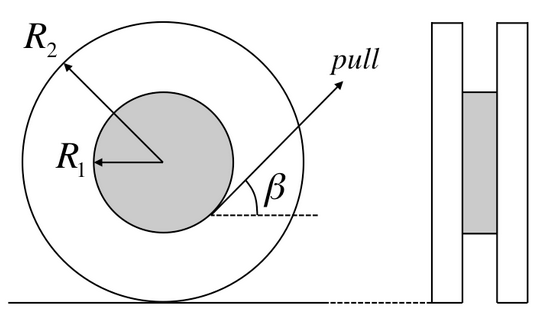
\includegraphics[scale=0.45]{Graphics/h7p5}
\end{center}

A yo-yo of mass $m$ rests on the floor (the static friction coefficient with the floor is $\mu$). The inner (shaded) portion of the yo-yo has a radius $R_1$, the two outer disks have radii $R_2$. A string is wrapped around the inner part. Someone pulls on the string at an angle $\beta$ (see sketch). The ``pull'' is very gentle, and is carefully increased until the yo-yo starts to roll without slipping. Try it at Home; it's Fun!

For what angles of $\beta$ will the yo-yo roll to the left and for what angles to the right?

\begin{enumerate}
\item Yo-Yo rolls to the left if $\displaystyle \sin \beta < \frac{R_1}{R_2}$, and to the right if $\displaystyle \sin \beta > \frac{R_1}{R_2}$.
\item Yo-Yo rolls to the left if $\displaystyle \sin \beta > \frac{R_1}{R_2}$, and to the right if $\displaystyle \sin \beta < \frac{R_1}{R_2}$.
\item Yo-Yo rolls to the left if $\displaystyle \cos \beta < \frac{R_1}{R_2}$, and to the right if $\displaystyle \cos \beta > \frac{R_1}{R_2}$.
\item Yo-Yo rolls to the left if $\displaystyle \cos \beta > \frac{R_1}{R_2}$, and to the right if $\displaystyle \cos \beta < \frac{R_1}{R_2}$.
\end{enumerate}

Hmm. Well, unfortunately I don't have a yo-yo (nor anything similar, like a spool of sewing thread), so I can't really try it out! I also have no real intuition of how it behaves here, though I do know that it rolls away when $\beta$ is large, and towards you when $\beta$ is small.

Since $\sin \beta \approx \beta$ for small angles, option 1 cannot be true; it is more likely to roll to the left if $\sin \beta$ is large.\\
Option 2 could be true.\\
$\cos \beta$ becomes smaller as the angle grows. Larger angle means more likely to roll to the left, so smaller cosine also means that. This means we can rule out option 4.

Left are options 2 and 3, though I don't see any obvious way to choose between the two without actually making the calculations! Let's have a look at that.

What can we say about the yo-yo? There are external forces, which also causes external torques. $R_1$ acts as a moment arm for our pull, for the torque relative to the center of the yo-yo.\\
There is also the force due to friction. Friction acts along $R_2$, and also causes a torque on the yo-yo, in the opposite direction to the torque due to the pull.

I will use a coordinate system where leftwards motion is positive.

If we draw a free-body diagram (considering only the center of mass; we should not do this for torques, since distances matter there) and use $P$ to notate the force due to our pull, we find $P \cos \beta$ in the rightwards direction (negative, in this coordinate system), and $F_{fr}$ towards the left.

Using Newton's second law, we can write for the center of mass,

\begin{equation}
m a_{cm} = F_{fr} - P \cos \beta
\end{equation}

We can then calculate the torque due to this pulling force, as $\vec{R} \times \vec{P}$; the angle to the position vector is always 90 degrees, and $\vec{R}$, the moment arm, is $R_1$, since the string is wrapped around $R_1$:

\begin{equation}
\tau_P = R_1 P \text{ (direction: out of the screen / causes CCW rotation)}
\end{equation}

There is also a torque due to friction. Again, the angle is always 90 degrees, so $\vec{R} \times \vec{F_{fr}}$ is just the magnitude of the two multiplied together, where the moment arm is now $R_2$ (friction acts on the outside of the yo-yo):

\begin{equation}
\tau_{fr} = R_2 F_{fr} \text{ (direction: in to the screen / causes CW rotation)}
\end{equation}

When $\tau_{fr} > \tau_P$, there is clockwise rotation, and the yo-yo rolls towards the right. When $\tau_P$ wins, it moves towards the right.\\
Since the torque must reverse direction between these two cases, there is also the possibility that the net torque is zero.

Net torque (CCW/left): $\tau = \tau_P - \tau_{fr} = R_1 P - R_2 F_{fr}$

Using the condition that the torque is zero, we can relate $F_{fr}$ to $P$:

\begin{align}
R_1 P - R_2 F_{fr} &= 0\\
F_{fr} &= \frac{R_1}{R_2} P
\end{align}

Making this substitution into the Newton's second law equation:

\begin{equation}
a = \frac{P}{m} \left(\frac{R_1}{R_2} - \cos \beta\right)
\end{equation}

This acceleration is positive when the yo-yo accelerates to the left, due to the choice of coordinate system, so the condition for moving towards the left is that the above expression is greater than zero. We set up the inequality and solve:

\begin{equation}
\frac{P}{m} \left(\frac{R_1}{R_2} - \cos \beta\right) > 0
\end{equation}

That happens when

\begin{equation}
\frac{R_1}{R_2} > \cos \beta
\end{equation}

which of course is the same as one of the answer options,

\begin{equation}
\cos \beta < \frac{R_1}{R_2}
\end{equation}

So the answer is option 3,\\
Yo-Yo rolls to the left if $\displaystyle \cos \beta < \frac{R_1}{R_2}$, and to the right if $\displaystyle \cos \beta > \frac{R_1}{R_2}$.

\section{Problem 6: Stick on table}

``A uniform stick of mass $m$ and length $\ell$ is suspended horizontally with end B at the edge of a table as shown in the diagram, and the other end A is originally held by hand.\\
The hand at A is suddenly released.

\begin{center}
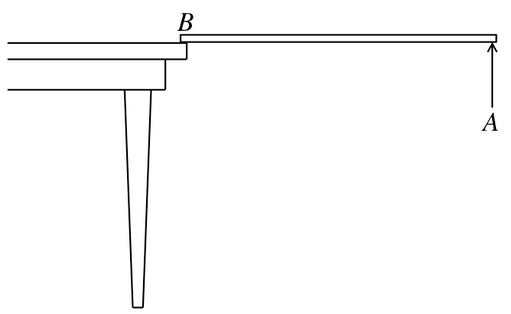
\includegraphics[scale=0.45]{Graphics/h7p6}
\end{center}

At the instant immediately after the release:

(a) What is the magnitude of the torque ($\tau_B$) about the end B at the edge of the table? Express your answer in terms of $m$, $\ell$ and acceleration due to gravity $g$ as needed.\\
(b) What is the magnitude of the angular acceleration $\alpha$ about the end B at the edge of the table? Express your answer in terms of $m$, $\ell$ and acceleration due to gravity $g$ as needed.\\
(c) What is the magnitude of the vertical acceleration a of the center of mass? Express your answer in terms of $m$, $\ell$ and acceleration due to gravity $g$ as needed.\\
(d) What is the magnitude of the vertical component of the hinge force (N) at B? Express your answer in terms of $m$, $\ell$ and acceleration due to gravity $g$ as needed.''

Torque is the force times the moment arm length, which is easy in this case. The relevant force is $m g$, which acts on the center of mass. Since the stick is uniform, the center of mass is at $\frac{\ell}{2}$. The torque relative to point B is simply

\begin{equation}
\tau_B = m g \frac{\ell}{2}
\end{equation}

since the angle between the two vectors is 90 degrees (just after the stick is released).

We can now find the angular acceleration by knowing the torque, via $\tau = I \alpha$. The moment of inertia in question is the one for the rod, about its end, since that is the pivot point.\\
Since the pivot point is clearly not at the center of mass in this case, we need to use the parallel axis theorem.

I remember that $I_c = \frac{1}{12} m \ell^2$ for a rod, but we then need to add a term due to the parallel axis theorem. The distance between the center of mass and this new axis is half the rod's length, so via the parallel axis theorem,

\begin{equation}
I_B = \frac{1}{12} m \ell^2 + m \left(\frac{\ell}{2}\right)^2
\end{equation}

Now, using $\tau_B = I_B \alpha$, we can solve for $\alpha$:

\begin{align}
m g \frac{\ell}{2} = \alpha\left( \frac{1}{12} m \ell^2 + m \left(\frac{\ell}{2}\right)^2 \right)\\
g \frac{\ell}{2} = \alpha \frac{1}{12} \ell^2 + \alpha \frac{\ell^2}{4}\\
g = \alpha \frac{1}{6} \ell + \alpha \frac{\ell}{2}\\
g = \alpha\ell \left( \frac{1}{6} + \frac{1}{2}\right)\\
\frac{g}{\ell} = \alpha \left( \frac{4}{6}\right)\\
\frac{3g}{2\ell} = \alpha
\end{align}

Next, they want to know the vertical acceleration of the center of mass. $\alpha$ describes the angular acceleration about point B, that the center of mass undergoes. We can use the relationship $a = \alpha R$, and in this case, $R = \frac{\ell}{2}$.

\begin{equation}
a = \frac{3g}{2\ell} \frac{\ell}{2}
\end{equation}
\begin{equation}
a = \frac{3g}{4}
\end{equation}

Finally, what is the magnitude of the vertical component of the hinge force at B?\\
Well, first up, what is hinge force? I haven't seen that term before, but I assume it is the normal force from the table on the end of the stick, especially as they give it as $N$.

It's clearly not zero, or the stick would just fall right through.\\
What we do here is to remember the videos and demonstration of an impulse on a ruler. No matter \emph{where} on the ruler the force is exerted, the acceleration of the center of mass is affected in the same way. Therefore, we can use Newton's second law to relate the net downwards force, $m g - N$, with the mass times acceleration of the stick:

\begin{align}
m g - N &= m a\\
N &= m(g - a)
\end{align}

We know $a$ from above, so we can substitute than in there:

\begin{align}
N &= m(g - \frac{3g}{4})\\
N &= \frac{m g}{4}
\end{align}

\section{Problem 7: Physical pendulum}

``A physical pendulum consists of a disc of radius $R$ and mass $m$ fixed at the end of a rod of mass $m$ and length $\ell$.

\begin{center}
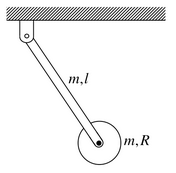
\includegraphics[scale=0.8]{Graphics/h7p7}
\end{center}

(a) Find the period of the pendulum for small angles of oscillation. Express your answer in terms of $m$, $R$, $\ell$ and acceleration due to gravity $g$ as needed.\\
(b) For small angles of oscillation, what is the new period of oscillation if the disk is mounted to the rod by a frictionless bearing so that it is perfectly free to spin? Express your answer in terms of $m$, $R$, $\ell$ and acceleration due to gravity $g$ as needed.''

This one took me a while, in large part because of a silly math error that I didn't spot for an hour or so... An $\ell$ disappeared when I added two expressions. Very frustrating!

Anyway. In part (a), the disk is fixed. We begin by calculating the total moment of inertia for rotating about what I will call point P, the point where the rod is mounted to the roof.

For the rod, we use the parallel axis theorem:

\begin{equation}
I_{rod,end} = \frac{1}{12} m \ell^2 + m \left(\frac{\ell}{2}\right)^2 = \frac{m \ell^2}{3}
\end{equation}

We also use the parallel axis theorem for the disc. About the disc's own center of mass, $I_{cm} = \frac{1}{2} m R^2$. We need to add to that the distance to the new axis, which is $\ell$ away.

\begin{equation}
I_{disc} = \frac{1}{2} m R^2 + m \ell^2 = m \left( \frac{R^2}{2} + \ell^2 \right)
\end{equation}

The total moment of inertia for rotation about the pivot point, for the combination is then

\begin{equation}
I_P = \frac{1}{6} m (8 \ell^2 + 3 R^2)
\end{equation}

Let's now consider the torque (relative to the pivot point, P). There is a torque due to the rod (because of gravity acting on its center of mass), and a torque due to the wheel (again, due to gravity acting on its center of mass). These torques depend on the moment arm length, the force of gravity, and the sine of the angle between the two, via the cross product definition:

\begin{align}
\tau_{P,rod}  &= \vec{r_P} \times \vec{F_g} = \frac{\ell}{2} m g \sin \theta\\
\tau_{P,disc} &= \vec{r_P} \times \vec{F_g} = \ell m g \sin \theta\\
\tau_P        &= \tau_{P,rod} + \tau_{P,disc} = \frac{3}{2} m g \ell \sin \theta
\end{align}

This is a restoring torque, that is always trying to get things back to equilibrium. Using Newton's second law, or perhaps rather its rotational equivalent $\tau = I \alpha$, only with a negative sign in front since it is a restoring torque:

\begin{equation}
\alpha = -\frac{3}{2 I_P} m g \ell \sin \theta
\end{equation}

Using $\alpha = \ddot{\theta}$, and a small angle approximation $\sin \theta \approx \theta$, we get

\begin{equation}
\ddot{\theta} + \frac{3}{2 I_P} m g \ell \theta = 0
\end{equation}

... which is simple harmonic oscillator. This is of course what we wanted all along. The period is then given by $\displaystyle \frac{2 \pi}{\omega}$, where $\omega^2$ is the stuff multiplying the square root. We flip that upside down, take the square root, and multiply by the $2 \pi$:

\begin{equation}
T = \frac{2 \pi}{\omega} = 2 \pi \sqrt{\frac{2 I_P}{3 m g \ell}}
\end{equation}

\begin{align}
T &= 2 \pi \sqrt{\frac{m (8 \ell^2 + 3 R^2))}{9 m g \ell}}\\
                         &= \frac{2\pi}{3} \sqrt{\frac{8 \ell^2 + 3 R^2}{g \ell}}
\end{align}

What happens for part (b)? When the disc is free to spin, it is also free to stay stationary, so to speak. 
That is, when it is \emph{fixed}, it is \emph{forced} to rotate along with the motion. If we made a vertical mark at the top of the disk, that mark would turn at an angle $\theta$ together with the rod and the rest of the disc.\\
Because of this, it has a spin component of moment of inertia of $I_{cm,disk} = \frac{1}{2} m R^2$, in addition to the orbital component of $m R^2$.

With a frictionless bearing, on the other hand, that vertical mark on the disk would be vertical at all times, which means it is not spinning any more.\\
There is no torque acting on the disc: gravity acts equally on all points, and since it is attached in the center with \emph{no friction}, there can be no torque due to the pin there, either.

This means that the term for the disc's moment of inertia that is due to the spin disappears, and $I_{disc} = m R^2$ -- only the orbital part remains.\\
So we can think of the motion of the disc as having two components: one ``orbital'', and one ``spin''. In the previous case, both were present. In this case, when the disc can stay stationary (have no spin motion at all), only the orbital motion remains, and so only the orbital part of the moment of inertia remains.

The torque is unchanged, since we calculated that based on the center of mass. What changes is $I_P$; the part due to the rod is unchanged, but that due to the disc changes, so that

\begin{equation}
I_{disc} = m \ell^2
\end{equation}

The total moment of inertia about the pivot point is again the sum of the two moments of inertia:

\begin{equation}
I_P = \frac{m \ell^2}{3} + m \ell^2 = \frac{4 m \ell^2}{3}
\end{equation}

That is the only thing that changes, so we stick that into the equation for the period:

\begin{equation}
T = \frac{2 \pi}{\omega} = 2 \pi \sqrt{\frac{2 I_P}{3 m g \ell}}
\end{equation}

\begin{align}
T &= 2 \pi \sqrt{\frac{2 (\frac{4m \ell^2}{3})}{3 m g \ell}}\\
T &= 2 \pi \sqrt{\frac{8m \ell^2}{9 m g \ell}}\\
T &= \frac{2 \pi}{3} \sqrt{\frac{8 \ell}{g}}
\end{align}

That solves this problem!

\section{Problem 8: Two rotating disks}

``A solid disk 1 with radius $R_1$ is spinning freely about a frictionless horizontal axle $\ell$ at an angular speed $\omega$ initially. The axle $\ell$ is perpendicular to disk 1, and goes through the center S of disk 1.

The circumference of disk 1 is pushed against the circumference of another disk (disk 2). Disk 2 has the same thickness and density as disk 1, but has a radius $R_2$, and it is initially at rest. Disk 2 can rotate freely about a horizontal axle $m$ through its center P. Axles $m$ and $\ell$ are parallel. The friction coefficient between the two touching surfaces (disk circumferences) is $\mu$.

We wait until an equilibrium situation is reached (i.e. the circumferences of the two disks are no longer slipping against each other). At that time, disk 1 is spinning with angular velocity $\omega_1$, and disk 2 is spinning with angular velocity $\omega_2$.

\begin{center}
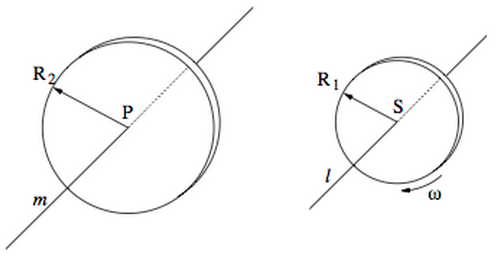
\includegraphics[scale=0.8]{Graphics/h7p8}
\end{center}

Calculate the magnitude of the angular velocities $|\omega_1|$ and $|\omega_2|$ in terms of $R_1$, $R_2$ and $\omega$.

It is quite remarkable that $\omega_1$ and $\omega_2$ are independent of $\mu$, and it is also independent of the time it takes for the equilibrium to be reached (i.e independent of how hard one pushes the disks against each other).''

Unlike most cases, I'm writing almost all the text for this problem after having solved it. (I usually write while solving, then clean up the text when I have everything correct, and feel I understand the solution fully.)\\
This problem was certainly the most confusing of the week for many, including myself until I thought about it for quite a long while, while following the forum discussions.

First: angular momentum will \emph{not be conserved}! This is an extremely important point, of course -- solving this by assuming it \emph{is} conserved does not work. (Except a side note, below.)

It is clear that there is friction between the disks, or they could not affect one another. Friction is proportional to the normal force, but since the disks are at the side of one another, there is no natural force to push them together.\\
This force must be provided by something \emph{external} to the system, such as a person holding the two axles.\\
In addition, the force due to friction acts ``upwards'' and ``downwards'' on the two disks, respectively (in the order shown in the figure). With a net force upwards or downwards on an object, the center of mass must accelerate upwards! $\displaystyle a_{cm} = \frac{F_{ext}}{m}$ must hold for the center of mass. Therefore, in order for the disks to stay where they are, another \emph{external force} comes in: the leftwards disk must be forced down, and the rightwards disk must be forced up, or they will not stay put.

Now, in a bit of a freak coincidence, the correct solution \emph{can} be found by assuming angular momentum is conserved, and by assuming that $\displaystyle \frac{m_1}{m_2} = \frac{R_1}{R_2}$, which is incorrect! Since mass is proportional to volume, and volume is $\pi R_i^2 h$, the correct equation is $\displaystyle \frac{m_1}{m_2} = \frac{R_1^2}{R_2^2}$.

Combining this \emph{correct} equation with conservation of momentum, and you can find an answer which looks like the correct ones, only that all exponents (on $R_1$ and $R_2$) are one too large! If you then also use the incorrect formula for the masses above, \emph{the error cancels out}, and you find the correct answer!\\
To be clear, this does not imply that the \emph{method} is correct -- it is trivial to show that the total angular momentum must change! See the end notes below, after my solution.

\subsection{My solution}

Okay, so let's consider this in more detail. To begin with, note that below, any time I say the leftmost disk, I mean the leftmost disk in the figure above, which is disk 2 (since it has radius $R_2$ and ends up spinning at $\omega_2$, I call it disk 2). The rightmost disk is disk 1.

Okay. First, we can write two equations regarding the change in angular momentum of each disk on its own. By the way, because we also deal with objects spinning about an axis through their center of mass, we don't need to specify the point relative to which we find the angular momentum, as the answer is the same for all such points.\\
The two equations relating these changes are

\begin{align}
\Delta L_1 &= I_1(\omega_1 - \omega)\\
\Delta L_2 &= I_2(\omega_2 - 0)
\end{align}

Disk 2 starts with 0 initial angular momentum, so its final angular momentum $I_2 \omega_2$ equals the change.

The most important forces involved will be the frictional forces due to the contact of the two disks. The magnitude of these forces is unknown (they depend on how hard the disks are pushed together, which we are not told), but that doesn't matter for the solution, as the problem sort-of states.

Disk 1 spins clockwise to begin with. When it comes in contact with disk 2, there is a frictional force on disk 1, due to disk 2. This frictional force must oppose the relative motion, and so it acts downwards (counterclockwise) on disk 1, slowing its rotation. (Anything else would be crazy!)\\
Via Newton's third law, there is an equal but opposite force on disk 2 (which is still stationary), due to disk 1. This means that force is upwards, i.e. causes counterclockwise rotation.

These forces must cause torque on the two disks, or their rotation would be unaffected (since torque causes change in rotational motion, just as force causes change in linear motion).\\
For disk 1, there is friction on the left side, acting downwards tangentially along the disk. The torque caused by this, relative to the disk's center, is the cross product of the position vector from the center and the friction vector:

\begin{equation}
\tau_1 = \vec{R_1} \times \vec{F_{fr}} = -R_1 F_{fr}
\end{equation}

As for direction, via the right-hand rule, it is out of the screen, i.e. acts counterclockwise. Again, anything else would be crazy, since the opposite torque would speed the disk's rotation up.\\
I notate this with a minus sign, as I use clockwise rotation (into the screen) as positive. That is the initial rotation, so I figured it would make sense to call that positive.

For disk 2, we do the same process. Friction is on the right side, acting upwards, tangentially. The torque relative to this disk's center is

\begin{equation}
\tau_2 = \vec{R_2} \times \vec{F_{fr}} = -R_2 F_{fr}
\end{equation}

The direction of this torque is also out of the screen, i.e. it acts counterclockwise. This is also clear if you consider the direction of the motion; the disk starts to spin such that the tangential velocity is reduced, so that slipping is reduced. This is only possible if it spins up counterclockwise.

Note that both torques act counterclockwise, which means angular momentum is increasing in the CCW direction for both disks, and therefore for the system of the two disks combined. This can clearly not be the case if angular momentum is conserved/held constant; if it were held constant, the increase in one disk must be matched by a decrease in the other.

I used $F_{fr}$ for both frictional forces, since they have the same magnitude via Newton's third law. Their directions do differ, however.

Say that this frictional force acts for an unknown time $\Delta t$. We can then also write the changes in angular momenta as

\begin{align}
\Delta L_1 &= - F_{fr} \Delta t R_1\\
\Delta L_2 &= - F_{fr} \Delta t R_2
\end{align}

using the relationship $\displaystyle \frac{dL}{dt} = \tau$, which becomes $\Delta L = \tau \Delta t$ if we bring it out of the differential form, and rearrange.

So, we have four equations; two per disk, both of which define the change in angular momentum. If we set them equal in pairs, we get two equations, with many unknowns ($F_{fr}$, $\Delta t$, $I_1$, $I_2$, $\omega_1$ and $\omega_2$ -- wow).\\
Not to worry, as we can eliminate many of those. First, we can eliminate $I_2$ by writing it in terms of $I_1$. It is specified that the disks have the same density and thickness, so we can relate their masses and/or moments of inertia by comparing the radii.

The mass of a disk with some density $\rho$ is $\pi R_i^2 h \rho$. The moment of inertia is then $\frac{1}{2} m R_i^2 = \frac{1}{2} (\pi R_i^2 h \rho) R_i^2$, and the ratio of the two moments of inertia becomes 

\begin{equation}
\frac{I_2}{I_1} = \frac{\frac{1}{2} (\pi R_2^2 h \rho) R_2^2}{\frac{1}{2} (\pi R_1^2 h \rho) R_1^2} = \frac{R_2^4}{R_1^4}
\end{equation}

which gives us $\displaystyle I_2 = I_1 \frac{R_2^4}{R_1^4}$. It is proportional to $R^4$ because both the mass and the moment of inertia are, on their own, proportional to $R^2$.

Combining the two pairs of $\Delta L$ equations, and making the substitution for $I_2$ using the relationship above, we have

\begin{align}
I_1 \omega_1 - I_1 \omega &= - F_{fr} \Delta t R_1\\
I_1 \frac{R_2^4}{R_1^4} \omega_2 &= - F_{fr} \Delta t R_2
\end{align}

We can divide the two equations -- note how this gets rid of $F_{fr}$, $\Delta t$ and $I_1$ all at once!

\begin{align}
\frac{I_1 \omega_1 - I_1 \omega}{I_1 \frac{R_2^4}{R_1^4} \omega_2} &= \frac{- F_{fr} \Delta t R_1}{- F_{fr} \Delta t R_2}\\
R_1^4 \frac{\omega_1 - \omega}{R_2^4 \omega_2} &= \frac{R_1}{R_2}\\
R_1^3 \frac{\omega_1 - \omega}{R_2^3 \omega_2} &= 1\\
R_1^3 \omega_1 - R_1^3 \omega &= R_2^3 \omega_2\\
R_1^3 \omega_1 - R_2^3 \omega_2 &= R_1^3 \omega
\end{align}

A bit of a prettier way to write this would be to consider the relative magnitudes of the two torques instead (the torques are \emph{not} the same in magnitude, but the frictional force that causes them \emph{are}). The end result is the same; it is simply a different way to write the equations.

Another relationship we can use is that of the linear velocities of the two disks, which need to match for there to be no slipping.

\begin{equation}
\omega_1 R_1 = -\omega_2 R_2
\end{equation}

We then have two equations and two unknowns:

\begin{align}
R_1^3 \omega_1 - R_2^3 \omega_2 &= R_1^3 \omega\\
\omega_1 R_1 &= -\omega_2 R_2
\end{align}

The solutions are

\begin{align}
\omega_1 &= \frac{R_1^2 \omega}{R_1^2 + R_2^2}\\
\omega_2 &= -\frac{R_1^3 \omega}{R_2 (R_1^2 + R_2^2)}
\end{align}

They asked for the magnitudes, though, so we need to drop the minus sign in front of $\omega_2$.

\subsection{Aftermath}

So with the solutions in mind, what happens in terms of angular momentum?

\begin{equation}
L_{initial} = I_1 \omega
\end{equation}
\begin{equation}
L_{final} = I_1 \omega_1 + I_2 \omega_2
\end{equation}

... keeping in mind that $\omega_2$ is negative. We know that $\omega > \omega_1$, and that the moments of inertia don't change. The change in angular momentum is

\begin{equation}
\Delta L_{sys} = L_{final} - L_{initial} =  (I_1 \omega_1 + I_2 \omega_2) - I_1 \omega
\end{equation}

Which is, using the expressions for the solutions $\omega_1$ and $\omega_2$, and using $\displaystyle I_2 = I_1 \frac{R_2^4}{R_1^4}$:

\begin{equation}
\Delta L_{sys} = -\frac{I_1 R_2^2 (R_1 + R_2)}{R_1 (R_1^2 + R_2^2)} \omega
\end{equation}

Not a very pretty expression (I think simplification might have made it uglier), but we can consider the simpler case when $R_2 = R_1$:

\begin{equation}
\Delta L_{sys,R_1=R_2} = -I_1 \omega
\end{equation}

In this special case, the change in angular momentum is exactly the negative of the \emph{initial} angular momentum: the net angular momentum is ZERO afterwards.\\
This does actually make a whole lot of sense. If the disks are identical (same thickness, radii and density implies same mass and same moment of inertia), they will rotate at the same angular speed... but opposite directions! Since $L_C = I_c \omega$, and both disks have the same magnitude (but opposite direction) of $\omega$, and the same $I_c$, the angular momentum of disk 1 is exactly the opposite of disk 1, and the sum is zero.

The solution for angular velocities in this special case is $\omega_1 = \omega/2$ and $\omega_2 = -\omega/2$, so.

\begin{equation}
L_{final,R_1=R_2} = I \frac{\omega}{2} + I \left(-\frac{\omega}{2}\right) = 0
\end{equation}

\section{Problem 9: Translation and rotation}

``A rod is lying at rest on a perfectly smooth horizontal surface (no friction). We give rod a short impulse (a hit) perpendicular to the length direction of the rod at X. The mass of the rod is 3 kg, and its length is 50 cm. The impulse is $\SI{4}{kg m/s}$. The distance from the center C of the rod to X is 15 cm.

(a) What is the translational speed $|\vec{v_{cm}}|$ of C after the rod is hit (in m/s)?\\
(b) What is the magnitude of the angular velocity $\omega$ of the rod about C (in rad/s)?\\
(c) How far (distance $D$ in meters) has the center C of the rod moved from its initial position 8 seconds after it was hit?\\
And what is the angle $\theta$ (in radians) between the direction of the rod at 8 seconds after it was hit, and its initial direction (before it was hit)? Give the smaller angle.\\
(d) What is the total kinetic energy $K$ of the rod after it was hit? (in joules)''

Hmm, this appears to be exactly as in the problem solving session. I will try to re-derive everything, though, since looking up the equations and entering the numbers doesn't teach you much.

The motion of the center of mass is very easy to derive. Say the rod is hit by an impulse $I$. It has zero momentum to begin with, so its new total momentum is $I$.\\
$\vec{p_{tot}} = m_{tot} \vec{v_{cm}}$ must hold, and so 

\begin{equation}
v_{cm} = \frac{I}{m} = \SI{4/3}{m/s}
\end{equation}

In the absence of external forces, this is held constant.\\
Part (c) is also extremely simple, then:

\begin{equation}
D = v_{cm} t = (\SI{4/3}{m/s})(\SI{8}{s}) = \SI{32/3}{m}
\end{equation}

The rotational motion is bit more tricky.\\
We can choose to consider torques relative to the center of mass, or relative to a point along the line of the impulse. (We \emph{can} choose differently, but why would we?)\\
I'm not sure which is easier in the end, but I find it easier to visualize it relative to the center of mass, point C.

The torque is then $\tau_C = F d$, where $F$ is the magnitude of the force, and $d$ the distance between C and X. It we multiply both sides by the (unknown) impact time, we get $\tau_C \Delta t = (F \Delta t) d$, which is the same as saying $L_C = I d$. The initial angular momentum relative to point C is zero, so this is the total angular momentum after the hit.

The angular momentum relative to point C is about the center of mass; so $L_C = I_c \omega$ also holds (where $I_c$ is the moment of inertia of the rod around the center). Setting the two equal,

\begin{equation}
I_c \omega = I d
\end{equation}
\begin{equation}
\omega = \frac{I d}{I_c} = \frac{I d}{\frac{1}{12} m \ell^2}
\end{equation}

For the numbers given, $\omega = 9.6$ rad/s.

After 8 seconds, it has rotated 76.8 radians, which about 12.22 rotations; the angle should be a bit less than 90 degrees (0.22 radians), in other words.\\
To find the angle,

\begin{equation}
\theta = 76.8 \bmod (2 \pi) = \SI{1.402}{rad} = \ang{80.32}
\end{equation}

where $\bmod$ gives the remainder after a division. The result is the same as $76.8 - (2 \pi \times \lfloor \frac{76.8}{2 \pi} \rfloor)$.

Finally, the total kinetic energy. This is simply the sum of the translational (linear) kinetic energy, and the rotational:

\begin{equation}
K = \frac{1}{2} m v_{cm}^2 + \frac{1}{2} I_c \omega^2 = \SI{2.6667}{J} + \SI{2.88}{J} = \SI{5.5467}{J}
\end{equation}

\end{document}